\documentclass[11pt,a4paper]{article}
\usepackage[utf8]{inputenc}
\usepackage[margin=2cm]{geometry}
\usepackage{tikz}
\usetikzlibrary{shapes.geometric,arrows.meta,positioning,calc,fit,backgrounds,decorations.pathreplacing}
\usepackage{xcolor}
\usepackage{enumitem}
\usepackage{listings}
\usepackage{amsmath,amssymb}
\usepackage{booktabs}
\usepackage{hyperref}

\lstset{
    language=Python,
    basicstyle=\ttfamily\scriptsize,
    keywordstyle=\color{blue}\bfseries,
    commentstyle=\color{green!50!black},
    stringstyle=\color{red!70!black},
    numbers=left,
    numberstyle=\tiny\color{gray},
    breaklines=true,
    frame=single,
    backgroundcolor=\color{gray!5},
    showstringspaces=false
}

\definecolor{inputcol}{RGB}{52,152,219}
\definecolor{embedcol}{RGB}{155,89,182}
\definecolor{slotcol}{RGB}{46,204,113}
\definecolor{crosscol}{RGB}{26,188,156}
\definecolor{selfcol}{RGB}{22,160,133}
\definecolor{lstmcol}{RGB}{241,196,15}
\definecolor{outputcol}{RGB}{231,76,60}
\definecolor{bgcol}{RGB}{236,240,241}
\definecolor{physcol}{RGB}{230,126,34}

\title{\textbf{Pile Stiffness Degradation Model}\\[0.3cm]\large Slot-Attention Transformer --- Architecture \& Code}
\author{}
\date{}

\begin{document}
\maketitle

%===================================================
% PROBLEM (brief)
%===================================================
\section{Problem}

\textbf{Goal:} Given 8 soil/pile parameters, predict the full 44-step degradation of 3 stiffness values ($K_L$, $K_R$, $K_{LR}$).

\begin{itemize}[nosep]
    \item \textbf{Input:} 8 numbers --- PI, $G_{max}$, $\nu$, $D_p$, $T_p$, $L_p$, $I_p$, $D_p/L_p$
    \item \textbf{Output:} 3 curves $\times$ 44 steps --- lateral ($K_L$), rotational ($K_R$), cross-coupling ($K_{LR}$)
    \item \textbf{Data:} 19 scenarios from Excel (15 train, 4 test)
    \item \textbf{Physics:} $K_L, K_R$ always decrease; $K_{LR}$ can increase or decrease
\end{itemize}

%===================================================
% COMPLETE ARCHITECTURE
%===================================================
\section{Complete Architecture}

The model has 5 main stages:

\subsection*{Stage 1: Embedding}
The 8 input numbers are multiplied by a learned weight matrix to produce a vector of 64 numbers. This is called a \textbf{linear projection}. The 64-dimensional vector is then normalized (\texttt{LayerNorm} keeps values centered around 0 with stable variance) and passed through a \texttt{GELU} activation function (introduces non-linearity so the model can learn curved relationships, not just straight lines).

\subsection*{Stage 2: Slot Refinement ($\times 2$ iterations)}
The model has 21 \textbf{slots} --- 21 vectors of size 64 that are learned during training. Each slot specializes in encoding a different aspect of the output. The slots are refined in 2 rounds, each consisting of:

\begin{itemize}[nosep]
    \item \textbf{Cross-attention:} Each slot computes a weighted combination of the input embedding. The weights are determined by how relevant the input is to that slot. This uses 4 attention heads --- meaning the attention is computed 4 times independently with different learned weights, then the results are concatenated. The output is added back to the slot (residual connection) and normalized.
    \item \textbf{Self-attention:} Each slot computes a weighted combination of all other slots. This allows slots to coordinate and avoid redundancy. Same residual connection and normalization.
    \item \textbf{MLP:} Each slot is passed through a 2-layer feedforward network ($64 \to 128 \to 64$) with GELU activation and 10\% dropout (randomly zeroes 10\% of values during training to prevent overfitting). Same residual connection and normalization.
\end{itemize}

\subsection*{Stage 3: Slot Split}
After refinement, the 21 slots are split:
\begin{itemize}[nosep]
    \item \textbf{Slot 1} $\to$ passed through the \textbf{Initial Head} (a small network: $64 \to 32 \to 3$) to produce the 3 initial stiffness values ($K_L^0, K_R^0, K_{LR}^0$). Slot 1 is also used to set the starting memory of the LSTM ($h_0$ and $c_0$) via two linear projections.
    \item \textbf{Slots 2--21} $\to$ averaged into a single vector, then copied 43 times (one per remaining time step). A learned \textbf{positional embedding} is added to each copy so the decoder can distinguish step 2 from step 43. These 20 slots are also kept separately for use in decoder cross-attention.
\end{itemize}

\subsection*{Stage 4: LSTM Decoder}
The LSTM (Long Short-Term Memory) is a recurrent network with 2 stacked layers. It processes the 43 input vectors one at a time sequentially, maintaining an internal hidden state that carries information from previous steps. At each step it outputs a 64-dimensional vector. Its hidden state is initialized from Slot 1 (not from zeros), so it starts with knowledge of the specific pile.

After the LSTM, each of the 43 output vectors goes through \textbf{decoder cross-attention}: each output computes a weighted combination of the 20 drop slots (Slots 2--21). This lets each time step selectively use the most relevant drop slot information. The result is added to the LSTM output (residual) and normalized.

\subsection*{Stage 5: Drop Head + Physics + Output Assembly}
Each of the 43 refined vectors is projected from 64 dimensions to 3 values ($\Delta K_L$, $\Delta K_R$, $\Delta K_{LR}$) via the \textbf{Drop Head} ($64 \to 32 \to 3$).

\textbf{Physics constraint:} $K_L$ and $K_R$ always degrade, so their drops are forced negative by applying $d = -|d|$. $K_{LR}$ can go either direction, so it is left unconstrained.

The final output is assembled by cumulative summation:
$$K(t) = K^0 + \sum_{n=1}^{t-1} d_n$$
Step 1 is the initial value $K^0$, and each subsequent step adds one more drop. The result is a tensor of shape $[B, 44, 3]$.

\begin{center}
\resizebox{\textwidth}{!}{%
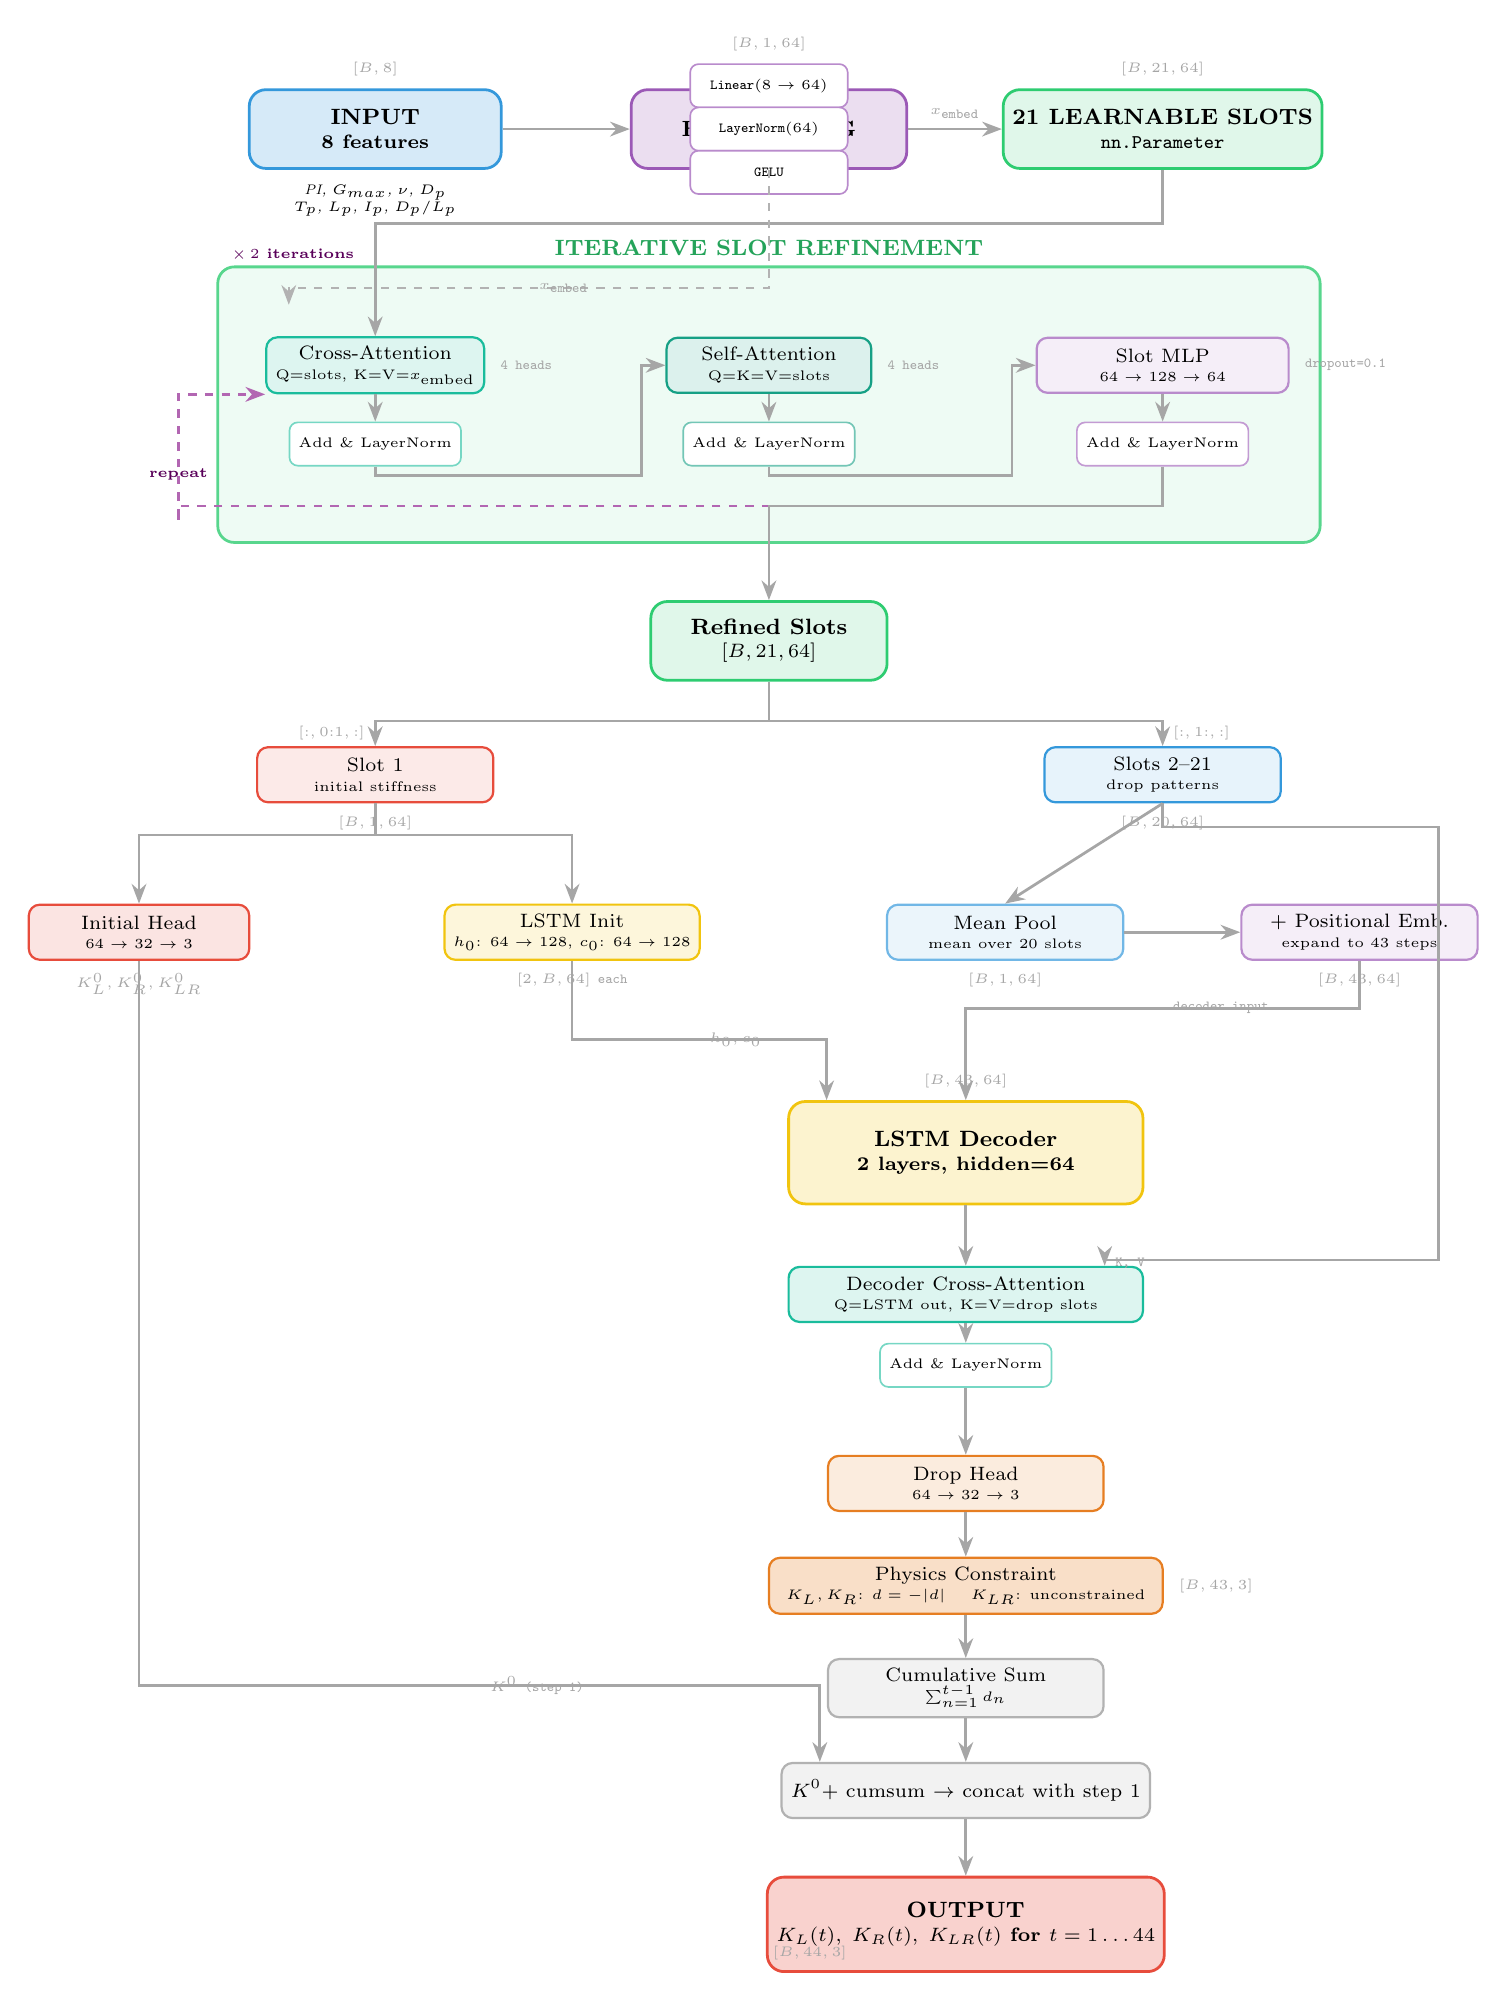
\begin{tikzpicture}[
    >={Stealth[length=2.5mm]},
    block/.style={rectangle, rounded corners=6pt, minimum width=3.2cm, minimum height=1cm, align=center, font=\footnotesize\bfseries, draw, line width=1pt},
    smallblock/.style={rectangle, rounded corners=4pt, minimum width=2.6cm, minimum height=0.7cm, align=center, font=\scriptsize, draw, line width=0.8pt},
    tinyblock/.style={rectangle, rounded corners=3pt, minimum width=2cm, minimum height=0.55cm, align=center, font=\tiny, draw, line width=0.6pt},
    arrow/.style={->, thick, gray!70, line width=1pt},
    darrow/.style={->, thick, line width=1pt},
    dashedarrow/.style={->, dashed, gray!60, line width=0.8pt},
    note/.style={font=\tiny\itshape, align=center, text width=2.2cm},
    dimlab/.style={font=\tiny\ttfamily, text=gray!70},
    looplab/.style={font=\tiny\bfseries, text=violet!70!black},
]

% ============================================================
% ROW 1: INPUT -> EMBEDDING -> SLOT INIT
% ============================================================

% Input
\node[block, fill=inputcol!20, draw=inputcol] (inp) at (0,0)
    {INPUT\\[-1pt]{\scriptsize 8 features}};
\node[note, below=2pt of inp] {PI, $G_{max}$, $\nu$, $D_p$\\$T_p$, $L_p$, $I_p$, $D_p/L_p$};
\node[dimlab, above=1pt of inp] {$[B, 8]$};

% Embedding
\node[block, fill=embedcol!20, draw=embedcol, minimum width=3.5cm] (emb) at (5,0)
    {EMBEDDING};
\node[tinyblock, fill=white, draw=embedcol!70] (emb1) at (5, 0.55) {\texttt{Linear}$(8 \to 64)$};
\node[tinyblock, fill=white, draw=embedcol!70] (emb2) at (5, 0) {\texttt{LayerNorm}$(64)$};
\node[tinyblock, fill=white, draw=embedcol!70] (emb3) at (5, -0.55) {\texttt{GELU}};
\node[dimlab, above=1pt of emb1] {$[B, 1, 64]$};

% Slot init
\node[block, fill=slotcol!15, draw=slotcol, minimum width=3.5cm] (slotinit) at (10,0)
    {21 LEARNABLE SLOTS\\[-1pt]{\scriptsize \texttt{nn.Parameter}}};
\node[dimlab, above=1pt of slotinit] {$[B, 21, 64]$};

\draw[arrow] (inp) -- (emb);
\draw[arrow] (emb) -- node[above, dimlab] {$x_{\text{embed}}$} (slotinit);

% ============================================================
% ROW 2: ITERATIVE REFINEMENT BLOCK (expanded)
% ============================================================

\node[block, fill=slotcol!8, draw=slotcol!80, minimum width=14cm, minimum height=3.5cm]
    (refine_box) at (5, -3.5) {};
\node[above=0pt of refine_box.north, font=\footnotesize\bfseries, slotcol!80!black]
    {ITERATIVE SLOT REFINEMENT};
\node[looplab, above right=-2pt and 2pt of refine_box.north west]
    {$\times\,2$ iterations};

% Cross-attention
\node[smallblock, fill=crosscol!15, draw=crosscol] (crossattn) at (0, -3)
    {Cross-Attention\\[-1pt]{\tiny Q=slots, K=V=$x_{\text{embed}}$}};
\node[tinyblock, fill=white, draw=crosscol!60] (crossnorm) at (0, -4)
    {Add \& LayerNorm};

% Self-attention
\node[smallblock, fill=selfcol!15, draw=selfcol] (selfattn) at (5, -3)
    {Self-Attention\\[-1pt]{\tiny Q=K=V=slots}};
\node[tinyblock, fill=white, draw=selfcol!60] (selfnorm) at (5, -4)
    {Add \& LayerNorm};

% MLP
\node[smallblock, fill=embedcol!10, draw=embedcol!70, minimum width=3.2cm] (mlp) at (10, -3)
    {Slot MLP\\[-1pt]{\tiny $64 \to 128 \to 64$}};
\node[tinyblock, fill=white, draw=embedcol!60] (mlpnorm) at (10, -4)
    {Add \& LayerNorm};

% Arrows inside refinement
\draw[arrow] (crossattn) -- (crossnorm);
\draw[arrow] (crossnorm) -- ++(0,-0.4) -| ($(selfattn.south west)-(0.3,0)$) |- (selfattn.west);
\draw[arrow] (selfattn) -- (selfnorm);
\draw[arrow] (selfnorm) -- ++(0,-0.4) -| ($(mlp.south west)-(0.3,0)$) |- (mlp.west);
\draw[arrow] (mlp) -- (mlpnorm);

% Dim labels
\node[dimlab, right=2pt of crossattn.east] {4 heads};
\node[dimlab, right=2pt of selfattn.east] {4 heads};
\node[dimlab, right=2pt of mlp.east] {dropout=0.1};

% Arrows from row 1 into refinement
\draw[arrow] (slotinit) -- ++(0,-1.2) -| (crossattn.north);
\draw[dashedarrow] (emb.south) -- ++(0,-1.5) -| ($(crossattn.north west)+(0.3,0.4)$)
    node[near start, right, dimlab] {$x_{\text{embed}}$};

% Loop arrow
\draw[dashedarrow, violet!60, line width=1pt]
    (mlpnorm.south) -- ++(0,-0.5) -| (-2.5, -5) |- (crossattn.south west)
    node[near start, below, looplab] {repeat};

% ============================================================
% ROW 3: SLOT SPLIT
% ============================================================

% Refined slots output
\node[block, fill=slotcol!15, draw=slotcol, minimum width=3cm] (refined) at (5, -6.5)
    {Refined Slots\\[-1pt]{\scriptsize $[B, 21, 64]$}};
\draw[arrow] (mlpnorm.south) -- ++(0,-0.5) -| (refined.north);

% Split
\node[smallblock, fill=outputcol!12, draw=outputcol, minimum width=3cm] (slot1) at (0, -8.2)
    {Slot 1\\[-1pt]{\tiny initial stiffness}};
\node[smallblock, fill=inputcol!12, draw=inputcol, minimum width=3cm] (slots220) at (10, -8.2)
    {Slots 2--21\\[-1pt]{\tiny drop patterns}};
\node[dimlab, below=1pt of slot1] {$[B, 1, 64]$};
\node[dimlab, below=1pt of slots220] {$[B, 20, 64]$};

\draw[arrow] (refined.south) -- ++(0,-0.5) -| (slot1.north)
    node[near end, left, dimlab] {$[:,0{:}1,:]$};
\draw[arrow] (refined.south) -- ++(0,-0.5) -| (slots220.north)
    node[near end, right, dimlab] {$[:,1{:},:]$};

% ============================================================
% ROW 4: TWO BRANCHES FROM SLOT 1, PLUS DROP SLOTS PATH
% ============================================================

% Initial Head
\node[smallblock, fill=outputcol!15, draw=outputcol, minimum width=2.8cm] (inithead) at (-3, -10.2)
    {Initial Head\\[-1pt]{\tiny $64 \to 32 \to 3$}};
\node[dimlab, below=1pt of inithead] {$K_L^0, K_R^0, K_{LR}^0$};

% h0/c0 projection
\node[smallblock, fill=lstmcol!15, draw=lstmcol, minimum width=2.8cm] (h0c0) at (2.5, -10.2)
    {LSTM Init\\[-1pt]{\tiny $h_0$: $64 \to 128$, $c_0$: $64 \to 128$}};
\node[dimlab, below=1pt of h0c0] {$[2, B, 64]$ each};

\draw[arrow] (slot1.south) -- ++(0,-0.4) -| (inithead.north);
\draw[arrow] (slot1.south) -- ++(0,-0.4) -| (h0c0.north);

% Mean aggregation
\node[smallblock, fill=inputcol!10, draw=inputcol!70, minimum width=3cm] (meanagg) at (8, -10.2)
    {Mean Pool\\[-1pt]{\tiny mean over 20 slots}};
\node[dimlab, below=1pt of meanagg] {$[B, 1, 64]$};

\draw[arrow] (slots220.south) -- (meanagg.north);

% Positional embedding + expand
\node[smallblock, fill=embedcol!10, draw=embedcol!70, minimum width=3cm] (posemb) at (12.5, -10.2)
    {+ Positional Emb.\\[-1pt]{\tiny expand to 43 steps}};
\node[dimlab, below=1pt of posemb] {$[B, 43, 64]$};

\draw[arrow] (meanagg) -- (posemb);

% ============================================================
% ROW 5: LSTM DECODER
% ============================================================

\node[block, fill=lstmcol!20, draw=lstmcol, minimum width=4.5cm, minimum height=1.3cm]
    (lstm) at (7.5, -13)
    {LSTM Decoder\\[-1pt]{\scriptsize 2 layers, hidden=64}};
\node[dimlab, above=1pt of lstm] {$[B, 43, 64]$};

\draw[arrow] (posemb.south) -- ++(0,-0.6) -| (lstm.north)
    node[near start, right, dimlab] {decoder input};
\draw[arrow] (h0c0.south) -- ++(0,-1.0) -| ($(lstm.north west)+(0.5,0)$)
    node[near start, right, dimlab] {$h_0, c_0$};

% ============================================================
% ROW 6: DECODER CROSS-ATTENTION
% ============================================================

\node[smallblock, fill=crosscol!15, draw=crosscol, minimum width=4.5cm] (deccross) at (7.5, -14.8)
    {Decoder Cross-Attention\\[-1pt]{\tiny Q=LSTM out, K=V=drop slots}};
\node[tinyblock, fill=white, draw=crosscol!60] (decnorm) at (7.5, -15.7)
    {Add \& LayerNorm};

\draw[arrow] (lstm) -- (deccross);
\draw[arrow] (deccross) -- (decnorm);

% Drop slots feed into decoder cross-attention
\draw[arrow] (slots220.south) -- ++(0,-0.3) -- ++(3.5,0) -- ++(0,-5.5)
    -| ($(deccross.north east)-(0.5,0)$)
    node[near end, right, dimlab] {K, V};

% ============================================================
% ROW 7: DROP HEAD + PHYSICS
% ============================================================

\node[smallblock, fill=physcol!15, draw=physcol, minimum width=3.5cm] (drophead) at (7.5, -17.2)
    {Drop Head\\[-1pt]{\tiny $64 \to 32 \to 3$}};

\draw[arrow] (decnorm) -- (drophead);

\node[smallblock, fill=physcol!25, draw=physcol, minimum width=5cm] (physics) at (7.5, -18.5)
    {Physics Constraint\\[-1pt]{\tiny $K_L, K_R$: $d = -|d|$ \quad $K_{LR}$: unconstrained}};

\draw[arrow] (drophead) -- (physics);
\node[dimlab, right=2pt of physics] {$[B, 43, 3]$};

% ============================================================
% ROW 8: CUMSUM + CONCAT -> OUTPUT
% ============================================================

\node[smallblock, fill=gray!10, draw=gray!60, minimum width=3.5cm] (cumsum) at (7.5, -19.8)
    {Cumulative Sum\\[-1pt]{\tiny $\sum_{n=1}^{t-1} d_n$}};

\draw[arrow] (physics) -- (cumsum);

\node[smallblock, fill=gray!10, draw=gray!60, minimum width=4cm] (concat) at (7.5, -21.1)
    {$K^0 +$ cumsum $\to$ concat with step 1};

\draw[arrow] (cumsum) -- (concat);

% Initial head feeds into concat
\draw[arrow] (inithead.south) -- ++(0,-9.2) -| ($(concat.north west)+(0.5,0)$)
    node[near start, right, dimlab] {$K^0$ (step 1)};

% Final output
\node[block, fill=outputcol!25, draw=outputcol, minimum width=5cm, minimum height=1.2cm]
    (output) at (7.5, -22.8)
    {OUTPUT\\[-1pt]{\scriptsize $K_L(t),\; K_R(t),\; K_{LR}(t)$ for $t = 1 \ldots 44$}};
\node[dimlab, above right=1pt and -1pt of output.south west] {$[B, 44, 3]$};

\draw[arrow] (concat) -- (output);

\end{tikzpicture}
}%
\end{center}

\textbf{Output formula:}
$$K(t) = \underbrace{K^0}_{\text{Slot 1 (initial head)}} + \sum_{n=1}^{t-1} \underbrace{d_n}_{\text{LSTM decoder (drop head)}} \qquad \text{where } d_n \leq 0 \text{ for } K_L, K_R$$

%===================================================
% FULL MODEL CODE
%===================================================
\section{Model Code}

\subsection{Model Definition (\texttt{\_\_init\_\_})}

This section defines all the layers and parameters of the model. Nothing is computed here --- it only creates the building blocks. Each \texttt{nn.Linear(a, b)} is a matrix of size $a \times b$ that will be learned during training. \texttt{nn.Parameter} creates a tensor that is also learned. \texttt{nn.MultiheadAttention} implements the attention mechanism described above. \texttt{nn.LSTM} implements the recurrent decoder.

\begin{lstlisting}
class SlotAttentionDegradation(nn.Module):
    def __init__(self, input_size, d_model=64, num_heads=4,
                 num_slots=21, max_seq_len=50, dropout=0.1,
                 num_iterations=2):
        super().__init__()
        self.num_iterations = num_iterations

        # PART 1: EMBEDDING -- project 8 inputs to 64 dimensions
        self.input_embed = nn.Sequential(
            nn.Linear(input_size, d_model),
            nn.LayerNorm(d_model),
            nn.GELU(),
        )

        # PART 2: 21 LEARNABLE SLOTS
        # Slot 1 = initial stiffness, Slots 2-21 = drop patterns
        self.slots = nn.Parameter(torch.randn(1, num_slots, d_model) * 0.02)

        # PART 3: CROSS-ATTENTION -- slots attend to the input
        self.cross_attn = nn.MultiheadAttention(d_model, num_heads,
                                                 dropout=dropout,
                                                 batch_first=True)
        self.cross_norm = nn.LayerNorm(d_model)

        # PART 4: SELF-ATTENTION -- slots attend to each other
        self.self_attn = nn.MultiheadAttention(d_model, num_heads,
                                                dropout=dropout,
                                                batch_first=True)
        self.self_norm = nn.LayerNorm(d_model)

        # PART 5: SLOT MLP -- per-slot feedforward (64 -> 128 -> 64)
        self.slot_mlp = nn.Sequential(
            nn.Linear(d_model, d_model * 2),
            nn.GELU(),
            nn.Dropout(dropout),
            nn.Linear(d_model * 2, d_model),
        )
        self.mlp_norm = nn.LayerNorm(d_model)

        # PART 6: INITIAL HEAD -- Slot 1 -> 3 initial values (KL, KR, KLR)
        self.initial_proj = nn.Sequential(
            nn.Linear(d_model, d_model // 2),  # 64 -> 32
            nn.GELU(),
            nn.Linear(d_model // 2, 3),        # 32 -> 3
        )

        # PART 7: LSTM INIT -- initialize h0, c0 from Slot 1
        self.h0_proj = nn.Linear(d_model, d_model * 2)
        self.c0_proj = nn.Linear(d_model, d_model * 2)

        # PART 8: POSITIONAL EMBEDDING -- learned per-step encoding
        self.pos_embed = nn.Parameter(
            torch.randn(1, max_seq_len, d_model) * 0.02)

        # PART 9: LSTM DECODER -- 2-layer LSTM, generates 43 drops
        self.seq_decoder = nn.LSTM(d_model, d_model, num_layers=2,
                                    batch_first=True, dropout=dropout)

        # PART 10: DECODER CROSS-ATTENTION -- LSTM output attends to drop slots
        self.decoder_cross_attn = nn.MultiheadAttention(
            d_model, num_heads, dropout=dropout, batch_first=True)
        self.decoder_cross_norm = nn.LayerNorm(d_model)

        # PART 11: DROP HEAD -- 64 -> 3 drop values per step
        self.drop_proj = nn.Sequential(
            nn.Linear(d_model, d_model // 2),  # 64 -> 32
            nn.GELU(),
            nn.Linear(d_model // 2, 3),        # 32 -> 3
        )
\end{lstlisting}

\newpage
\subsection{Forward Pass (\texttt{forward})}

This is the function that runs when data is passed through the model. It takes the 8 input values and returns 44 steps $\times$ 3 stiffness values. The steps match the architecture stages described above:
\begin{itemize}[nosep]
    \item Steps 1--3: embed input, expand slots, refine them in 2 iterations of cross-attention $\to$ self-attention $\to$ MLP.
    \item Step 4: split into Slot 1 (initial) and Slots 2--21 (drops).
    \item Steps 5--6: decode initial values from Slot 1 and use Slot 1 to initialize the LSTM's hidden state.
    \item Step 7: average the 20 drop slots, repeat 43 times, add positional embeddings.
    \item Steps 8--9: run the LSTM, then refine each output via cross-attention to the drop slots.
    \item Steps 10--11: project to 3 drops per step, apply physics ($-|d|$ for $K_L, K_R$), cumulative sum, prepend initial values.
\end{itemize}

\begin{lstlisting}
def forward(self, x, seq_len=None):
    batch_size = x.size(0)
    if seq_len is None:
        seq_len = self.pos_embed.size(1)

    # STEP 1: Embed input (8 -> 64)
    x_embed = self.input_embed(x).unsqueeze(1)  # [batch, 1, 64]

    # STEP 2: Expand slots for the batch
    slots = self.slots.expand(batch_size, -1, -1)  # [batch, 21, 64]

    # STEP 3: Iterative slot refinement (x2)
    for _ in range(self.num_iterations):
        # Cross-attention: slots attend to input
        cross_out, _ = self.cross_attn(slots, x_embed, x_embed)
        slots = self.cross_norm(slots + cross_out)

        # Self-attention: slots attend to each other
        self_out, _ = self.self_attn(slots, slots, slots)
        slots = self.self_norm(slots + self_out)

        # Feedforward + residual
        slots = self.mlp_norm(slots + self.slot_mlp(slots))

    # STEP 4: Split slots
    slot_initial = slots[:, 0:1, :]  # Slot 1 = initial stiffness
    slot_drops   = slots[:, 1:, :]   # Slots 2-21 = drop patterns

    # STEP 5: Decode initial values from Slot 1
    initial_decoded = self.initial_proj(slot_initial)  # [batch, 1, 3]

    # STEP 6: Initialize LSTM hidden state from Slot 1
    init_vec = slot_initial.squeeze(1)
    h0 = self.h0_proj(init_vec)
    h0 = h0.view(batch_size, 2, self.seq_decoder.hidden_size)
    h0 = h0.permute(1, 0, 2).contiguous()
    c0 = self.c0_proj(init_vec)
    c0 = c0.view(batch_size, 2, self.seq_decoder.hidden_size)
    c0 = c0.permute(1, 0, 2).contiguous()

    # STEP 7: Build LSTM input = mean of drop slots + positional encoding
    drop_agg = slot_drops.mean(dim=1, keepdim=True)
    drop_agg = drop_agg.expand(-1, seq_len-1, -1)
    decoder_input = drop_agg + self.pos_embed[:, :seq_len-1, :]

    # STEP 8: Run LSTM decoder (43 steps)
    lstm_out, _ = self.seq_decoder(decoder_input, (h0, c0))

    # STEP 9: Cross-attention -- LSTM output attends to drop slots
    refined, _ = self.decoder_cross_attn(
        lstm_out, slot_drops, slot_drops)
    refined = self.decoder_cross_norm(lstm_out + refined)

    # STEP 10: Project to 3 drops + apply physics constraint
    raw_drops = self.drop_proj(refined)           # [batch, 43, 3]
    drops_kl_kr = -torch.abs(raw_drops[:, :, :2]) # KL, KR forced negative
    drops_klr = raw_drops[:, :, 2:3]              # KLR unconstrained
    drops = torch.cat([drops_kl_kr, drops_klr], dim=2)

    # STEP 11: Cumulative sum to build the 44-step output
    cumulative = torch.cumsum(drops, dim=1)
    seq = initial_decoded + cumulative
    output = torch.cat([initial_decoded, seq], dim=1)  # [batch, 44, 3]

    return output
\end{lstlisting}

%===================================================
% DATA PIPELINE CODE
%===================================================
\newpage
\section{Data Pipeline Code}

Before training, the raw Excel data must be preprocessed:
\begin{itemize}[nosep]
    \item \textbf{Grouping:} Rows with the same 8 input values belong to the same pile scenario. The first row of each group is the initial stiffness. The remaining rows are the drops at each cycle. The actual stiffness at step $t$ is: $K(t) = K^0 - \sum_{n=1}^{t-1} \text{drop}_n$.
    \item \textbf{Input scaling:} \texttt{RobustScaler} subtracts the median and divides by the interquartile range (IQR = 75th percentile $-$ 25th percentile). It is more stable than standard scaling when the dataset is small (19 scenarios) because it is not affected by extreme values.
    \item \textbf{Output compression:} Stiffness values can be very large (e.g.\ $10^{11}$). The transformation $\text{sign}(y) \cdot \log(1 + |y|)$ compresses large magnitudes while preserving the sign. After compression, \texttt{RobustScaler} is applied again.
    \item \textbf{Split:} 15 scenarios for training, 4 for testing.
\end{itemize}

\begin{lstlisting}
# STEP 1: Load Excel data
df = pd.read_excel("REAL DATA.xlsx")
input_cols = ['PI', 'Gmax', 'v', 'Dp', 'Tp', 'Lp', 'Ip', 'Dp_Lp']

# STEP 2: Group rows by scenario (same 8 inputs = same pile)
for name, group in df.groupby(input_cols, sort=False):
    outputs = group[['kl', 'kr', 'klr']].values
    initial = outputs[0]                         # First row = initial values
    drops   = outputs[1:]                        # Remaining = drops
    actual  = initial - np.cumsum(drops, axis=0) # Cumulative degradation
    full_seq = np.vstack([initial, actual])      # 44-step sequence

# STEP 3: Scale inputs with RobustScaler (median-based, outlier-resistant)
scaler_X = RobustScaler()
X_scaled = scaler_X.fit_transform(X_array)

# STEP 4: Log-compress outputs then scale
# sign(y) * log1p(|y|) reduces large values while preserving sign
Y_log = np.sign(Y) * np.log1p(np.abs(Y))
scaler_Y = RobustScaler()
Y_scaled = scaler_Y.fit_transform(Y_log.reshape(-1, 3)).reshape(...)

# STEP 5: Train/test split -- 15 train, 4 test (80/20)
\end{lstlisting}

%===================================================
% TRAINING CODE
%===================================================
\section{Training Code}

Training repeats the following process for up to 3000 epochs:
\begin{enumerate}[nosep]
    \item Pass a batch of 4 scenarios through the model to get predictions.
    \item Compute 3 loss terms:
    \begin{itemize}[nosep]
        \item \textbf{Sequence loss} (Huber): the difference between predicted and real values across all 44 steps. Huber loss is less sensitive to outliers than MSE --- it uses squared error for small differences and linear error for large ones.
        \item \textbf{Initial value loss} (MSE $\times 3$): the squared error on step 1 only, multiplied by 3. This extra weight is needed because all subsequent steps are built on the initial value --- if step 1 is wrong, every step will be wrong.
        \item \textbf{Shape loss} (Huber on differences): instead of comparing raw values, this compares how much the curve changes between consecutive steps ($\text{pred}_{t+1} - \text{pred}_t$ vs.\ $\text{real}_{t+1} - \text{real}_t$). This forces the model to match the shape of the degradation curve.
    \end{itemize}
    \item Sum the 3 losses, compute gradients (\texttt{backward}), and update weights (\texttt{step}).
\end{enumerate}
\textbf{Optimizer:} AdamW with learning rate 0.0005 and weight decay 0.01. Weight decay adds a penalty proportional to the magnitude of the weights, which prevents the model from becoming too complex.

\textbf{Scheduler:} If the validation loss does not improve for 100 epochs, the learning rate is halved.

\textbf{Early stopping:} If no improvement for 300 epochs, training stops.

\begin{lstlisting}
model = SlotAttentionDegradation(input_size=8, d_model=64, num_heads=4,
                                  num_slots=21, max_seq_len=max_len,
                                  dropout=0.1, num_iterations=2)

optimizer = torch.optim.AdamW(model.parameters(), lr=0.0005,
                               weight_decay=0.01)
scheduler = ReduceLROnPlateau(optimizer, patience=100, factor=0.5)

huber = nn.SmoothL1Loss()  # Robust to outliers
mse   = nn.MSELoss()       # Mean squared error

for epoch in range(3000):
    model.train()
    for X_batch, Y_batch in train_loader:
        pred = model(X_batch, seq_len=max_seq_len)

        loss_seq  = huber(pred, Y_batch)                        # Full sequence loss
        loss_init = mse(pred[:, 0, :], Y_batch[:, 0, :]) * 3.0  # Initial value loss (x3)

        # Shape loss: compare step-to-step differences
        diff_pred   = pred[:, 1:, :] - pred[:, :-1, :]
        diff_target = Y_batch[:, 1:, :] - Y_batch[:, :-1, :]
        loss_shape  = huber(diff_pred, diff_target)

        loss = loss_seq + loss_init + loss_shape
        loss.backward()
        optimizer.step()

    # Early stopping after 300 epochs without improvement
\end{lstlisting}

%===================================================
% HYPERPARAMETERS & RESULTS
%===================================================
\section{Hyperparameters \& Results}

\begin{minipage}[t]{0.55\textwidth}
\renewcommand{\arraystretch}{1.2}
\begin{tabular}{@{}lc@{}}
\toprule
\textbf{Parameter} & \textbf{Value} \\
\midrule
$d_{\text{model}}$ (model dimension) & 64 \\
Attention heads & 4 \\
Slots (1 initial + 20 drops) & 21 \\
Slot refinement iterations & 2 \\
LSTM layers & 2 \\
Dropout & 0.1 \\
Batch size & 4 \\
Learning rate & 0.0005 \\
Weight decay (L2) & 0.01 \\
LR scheduler patience & 100 epochs \\
Early stopping patience & 300 epochs \\
Max epochs & 3000 \\
\bottomrule
\end{tabular}
\end{minipage}%
\hfill
\begin{minipage}[t]{0.38\textwidth}
\renewcommand{\arraystretch}{1.2}
\begin{tabular}{@{}lc@{}}
\toprule
\textbf{Output} & \textbf{R\textsuperscript{2}} \\
\midrule
$K_L$ (Lateral)       & 0.6799 \\
$K_R$ (Rotational)    & 0.7096 \\
$K_{LR}$ (Cross)      & 0.7042 \\
\midrule
\textbf{Overall}      & \textbf{0.7741} \\
\bottomrule
\end{tabular}

\vspace{0.5cm}
$R^2 = 1$ is perfect.\\
$R^2 = 0$ means no better than predicting the average.
\end{minipage}

%===================================================
% HOW TO USE
%===================================================
\section{How to Use}

\begin{enumerate}[nosep]
    \item \texttt{python train.py} --- trains model, saves \texttt{pile\_model.pth} + scalers + test data
    \item \texttt{python webapp.py} --- starts web server
    \item Open \texttt{http://127.0.0.1:5000} --- shows target vs.\ predicted curves for each test scenario
\end{enumerate}

\end{document}
